\section{Sobre o projeto}

A solução apresentada foi desenvolvida em um repositório do GitHub chamado ``filipecancio/sbc-template'' (figura~\ref{fig:fig10}) possuindo o template LaTex oficial da SBC (Sociedade Brasileira de Computação) para a produção de artigos. O acesso está disponível em ``https://github.com/filipecancio/sbc-template''. O repositório, ao ser acessado, se converte em um ambiente de desenvolvimento (Devcontainer), aonde não há necessidade de conhecimento em programação, basta editar qualquer arquivo ``.tex'' e é gerado um ``.pdf'' formatado no padrão SBC.

\begin{figure}[ht]
	\centering
	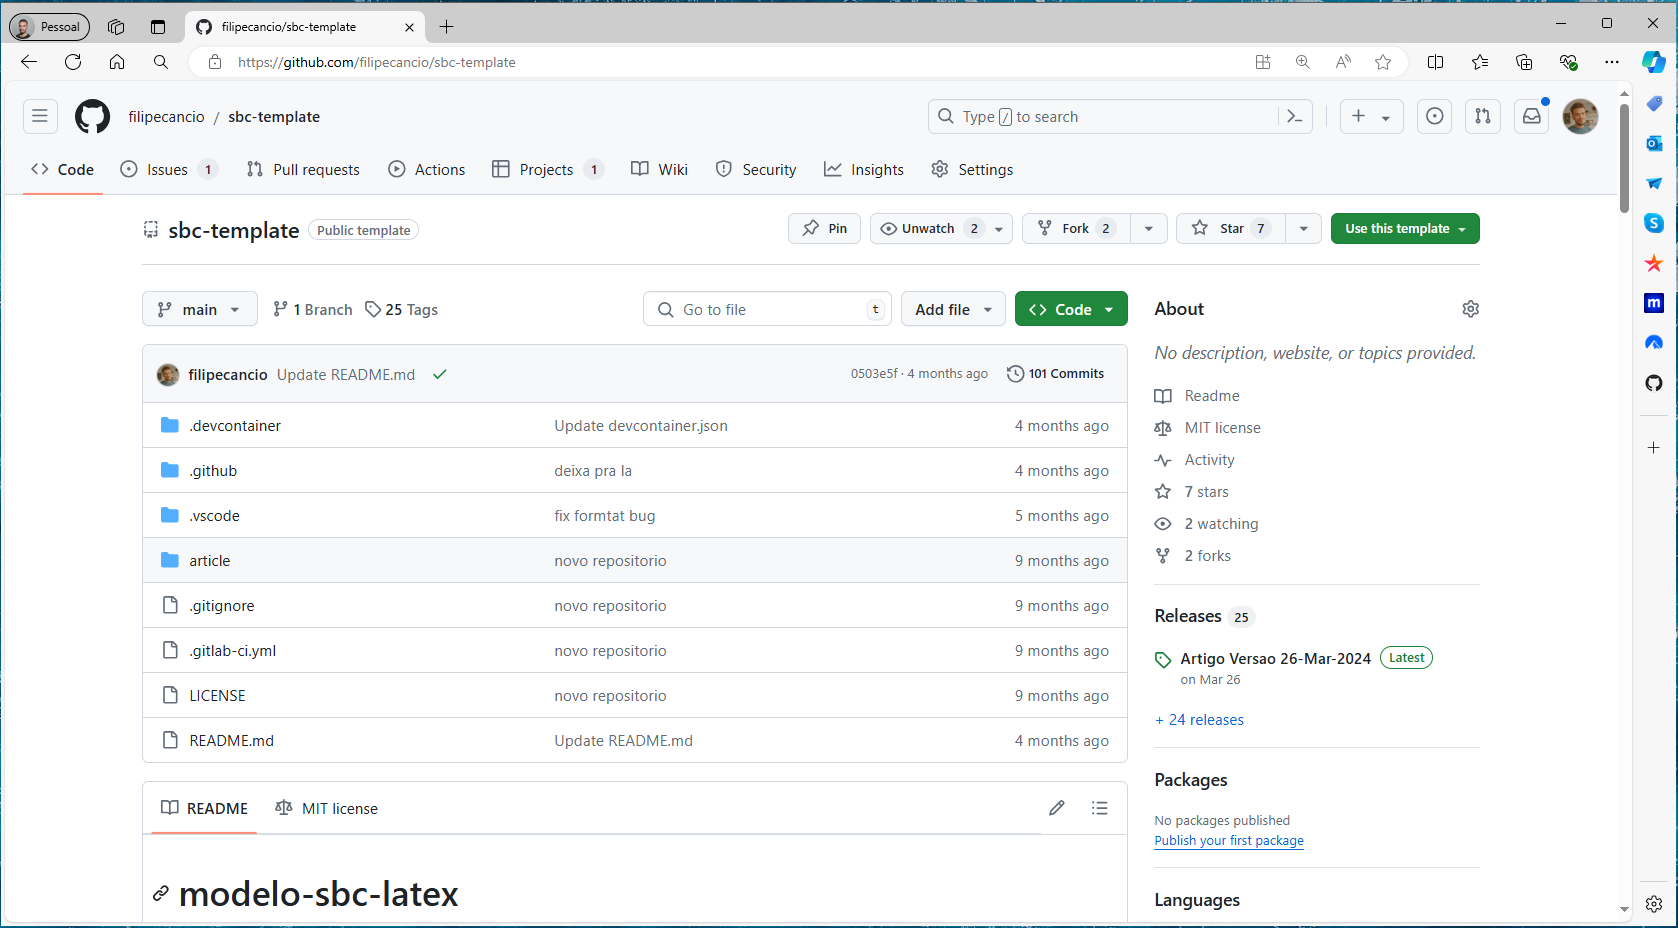
\includegraphics[width=.7\textwidth]{./images/fig10.png}
	\caption{Repositório filipe/sbc-template}
	\label{fig:fig10}
\end{figure}

\subsection{Funcionalidades}

Como solução alternativa às plataformas apresentadas anteriormente, o projeto possui algumas funcionalidades semelhantes porém, mais abrangentes e disponíveis de forma gratuita. Podemos visualizar abaixo um breve comparativo entre as plataformas.

\begin{table}[ht]
	\centering
	\begin{tabular}{|c|c|c|c|c|}
		\hline
		Plataformas & Usa LaTex & Colaborativo & Controle de versão & Sem Conexão
		\\
		\hline
		Overleaf & Sim & Limitado & Só na versao paga & Não \\
		\hline
		Microsoft Word & Não & Sim & Limitado & Sim \\
		\hline
		Google Documentos & Não & Sim & Limitado & Não \\
		\hline
		filipecancio/sbc-template & Sim & Sim & Sim & Sim \\
		\hline
	\end{tabular}
	\caption{Comparativos entre plataformas}
	\label{tab:tabela01}
\end{table}

Dentre as funcionalidades citadas acima (tabela~\ref{tab:tabela01}), podemos destacar as seguintes características do projeto ``filipecancio/sbc-template'':

\begin{itemize}
	\item Colaborativo: As ferramentas Word e Google Documentos utilizam serviços de nuvem (OneDrive e Drive, respectivamente) para compartilhar documentos. O Overleaf permite o compartilhamento com apenas uma conta e necessita de um plano pago para executar esse compartilhamento com mais diferentes contas. Já o projeto ``filipecancio/sbc-template'' utiliza as ferramentas do GitHub, que são gratuitas, para realizar o compartilhamento.
	\item Controle de versão: O Word e o Google Documentos possuem um controle de versão que permite apenas visualizar histórico de edições recentes de diferentes usuários. O Overleaf permite integração com GitHub e GitLab para controle de versão, porém precisa de um plano pago para habilitar a integração. O projeto ``filipecancio/sbc-template'' utiliza o controle de versão do Git (integrado ao GitHub), que possui toda uma estrutura para o desenvolvimento de software e essa estrutura é direcionada para o versionamento do artigo.
	\item Sem Conexão: O Word possui versão instalável permitindo o uso sem Conexão com rede, porém necessita de um plano pago. O Overleaf e o Google Documentos não possuem versão instalável e precisam de conexão com rede. O projeto ``filipecancio/sbc-template'' utiliza pode ser acessado por rede como usado com o Visual Studio Code instalado no computador para edição sem rede.
\end{itemize}

O projeto possui, além das caracteristícas acima, uma versatilidade para diferentes perfis de usuário. Mesmo voltado para iniciantes em LaTex e pessoas que não estão acostumadas com linguagens de programação, é útil para pessoas com conhecimento avançado nessa linguagem de marcação. 

O usuário deve possuir uma conta no GitHub para acessar o repositório ``filipecancio/sbc-template'', clonar com o nome desejado, de preferência com o nome do artigo, e começar a editar os arquivos de acordo ao manual de instruções disponível no arquivo ``README.md''.

As edições podem ocorrer de três formas:


\begin{itemize}
	\item Pelo  site do GitHub: Acessando pelo, você pode clicar diretamente nas pastas do diretório e nos arquivos correspondentes. O site permite a edição e dependendo da remificação escolhida, gera um ``.pdf'' após a edição~(figura~\ref{fig:fig01}).
	
	\begin{figure}[H]
		\centering
		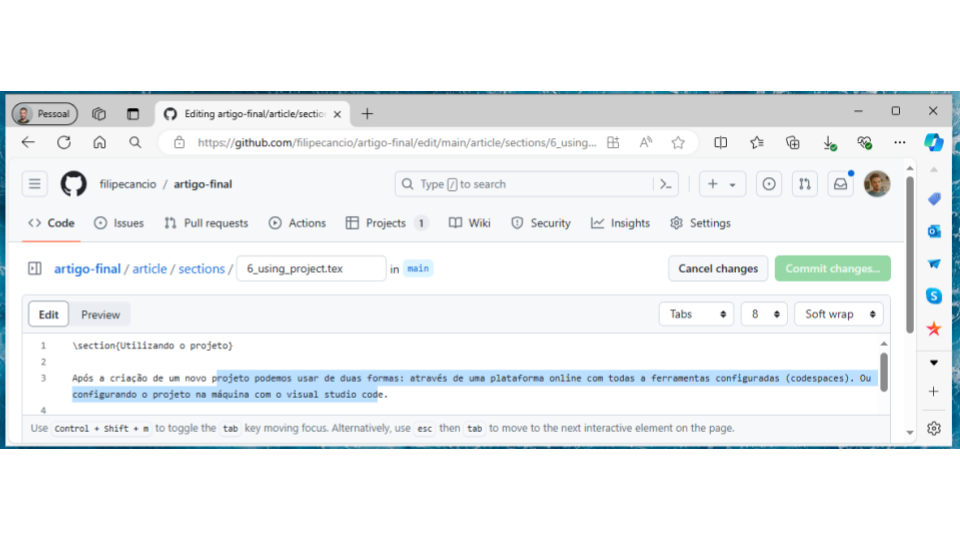
\includegraphics[width=.6\textwidth]{./images/fig03.png}
		\caption{Utilizando o projeto no site do GitHub}
		\label{fig:fig01}
	\end{figure}

	\item Pela plataforma Codespaces: O GitHub disponibiliza a edição  de forma mais completa utilizando o Codespaces, uma ferramenta que simula uma máquina e o Visual Code Studio no navegador, que pode ser acessada seguindo as instruções do repositório. O acesso pelo Codespaces permite o uso de todas funcionalidades de forma online (figura~\ref{fig:fig02}).
	
	\begin{figure}[H]
		\centering
		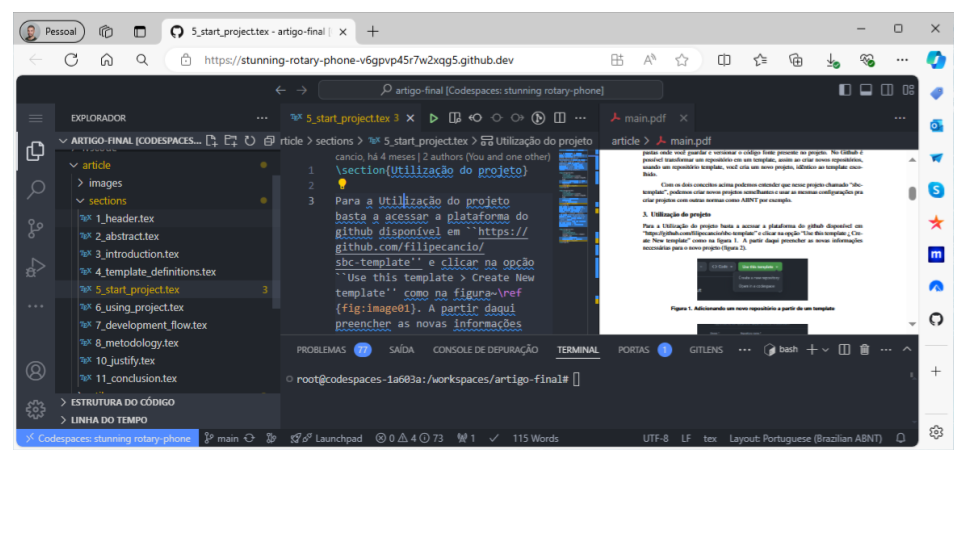
\includegraphics[width=.6\textwidth]{./images/fig02.png}
		\caption{Utilizando o projeto pelo Codespaces}
		\label{fig:fig02}
	\end{figure}

	\item Pelo Visual Studio Code: para o acesso sem rede, basta clonar o projeto seguindo as instruções no repositório e acessar o Visual Studio Code (figura~\ref{fig:fig03}).
	
	\begin{figure}[H]
		\centering
		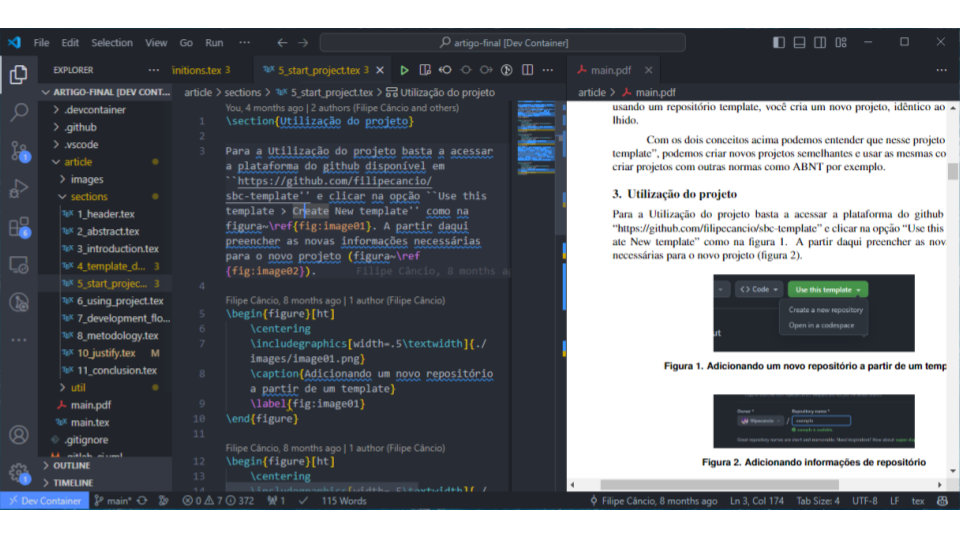
\includegraphics[width=.6\textwidth]{./images/fig01.png}
		\caption{Utilizando o projeto com Visual Studio Code}
		\label{fig:fig03}
	\end{figure}
\end{itemize}

Para tornar as formas de edições apresentadas mais intuitivas, o projeto possui um manual de instruções no arquivo ``README.md'' que orienta o usuário a editar o artigo. O manual é dividido em seções que explicam como clonar o projeto, editar o artigo, gerar o ``.pdf'' e subir as alterações para o GitHub. O manual também possui em cada seção vídeos tutoriais que mostram o passo a passo de cada ação, auxiliando usuários que não estão acostumados com a plataforma e possivelmente tenham dificuldade em seguir as intruções em texto.

Por ser desenvolvido no GitHub o versionamento é realizado utilizando o controle de versão Git. As instruções de versionamento no manual são voltadas para o básico de git apresentando apenas conceitos iniciais que podem ser usados diretamente no site ou com as ferramentas do Visual Studio Code e Codespaces.

\subsection{Destaques}
O projeto faz uso de três ferramentas do GitHub que valem a pena destacar. São estes: ``Versões'', Requisições de Pull e ``Projetos''.
\begin{itemize}
	\item ``Versões'': É possivel criar versões implementavéis e empacotadas de um projeto para o público. A ferramenta ``Versões'' disponibiliza todas as versões e seus respectivos empacotáveis em uma página com informações de novas funcionalides, data de submissão, autores, entre outros.~\cite{github:03}
	\item Requisições de Pull: Uma Requisição de Pull é uma página com propostas para mesclar as alterações feitas em uma remificação para outra~\cite{github:04}. No nosso projeto, as Requisições de Pull são utilizadas para correções e melhorias do artigo.
	\item ``Projetos'': É uma funcionalidade que integra Requisições de Pull afim de facilitar a gestão de projetos~\cite{github:05}.
\end{itemize}


No projeto ``filipecancio/sbc-template'' as versões implementavéis que as ``Versões'' carregam são arquivos no formato ``.pdf''. A cada nova edição, o projeto gera um novo ``.pdf'' com as alterações realizadas. A cada mudança gerada na ramificação de ``main'' é gerada uma versão com o ``.pdf'' datado (figura~\ref{fig:fig04}). Essa funcionalidade descarta qualquer necessidade de salvar versões de ``.pdf'', uma vez que o GitHub tem tudo salvo e documentado.
\begin{figure}[H]
	\centering
	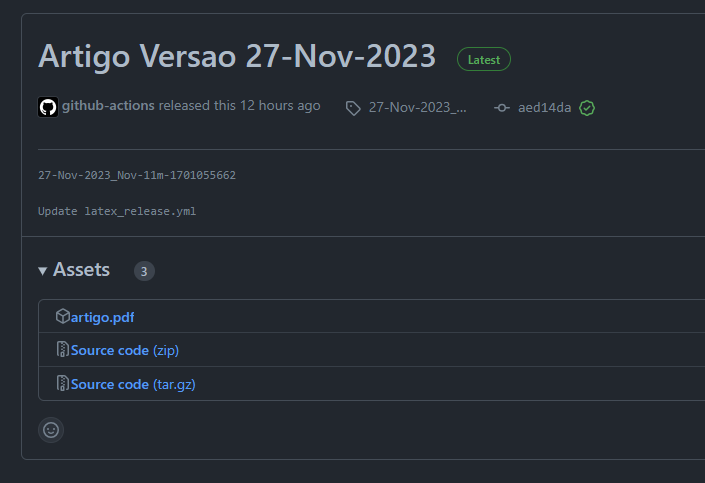
\includegraphics[width=.6\textwidth]{./images/fig04.png}
	\caption{Detalhes da ultima versão}
	\label{fig:fig04}
\end{figure}

Os artigos não precisam ser desenvolvidos na ramificações ``main''. O manual de instruções do projeto orienta que o pesquisador deve criar novas ramificações para implementar novos tópicos e correções. Associado a isso, pode ser utilizada a ferramenta de Requisições de Pull do GitHub para promover entre autor e orientador o controle das mudanças em cada versão, facilitando a correção dos artigos (figura~\ref{fig:fig05}). O uso de Requisições de Pull permite que o repositório gere versões de pdf exclusivas para aquela ramificação (figura~\ref{fig:fig06}).

\begin{figure}[H]
	\centering
	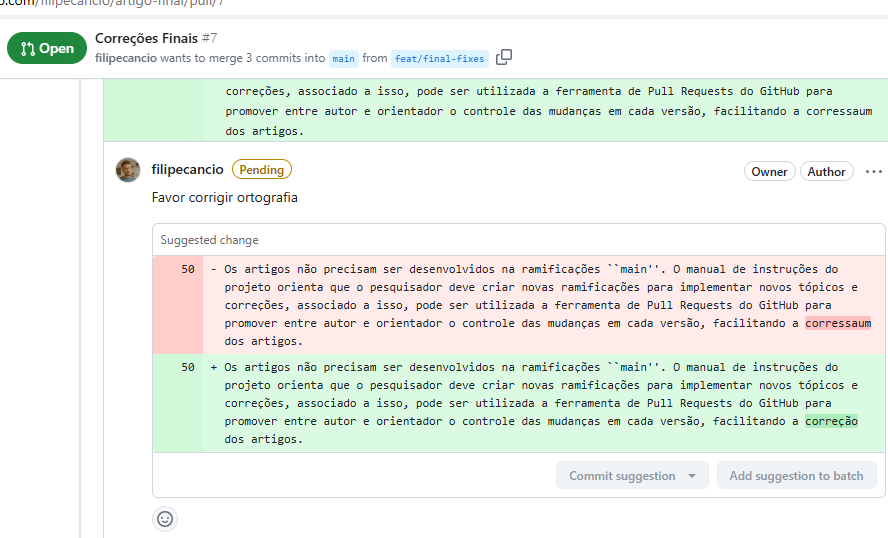
\includegraphics[width=.6\textwidth]{./images/fig05.png}
	\caption{Correção de trecho do artigo por Requisições de Pull}
	\label{fig:fig05}
\end{figure}

\begin{figure}[H]
	\centering
	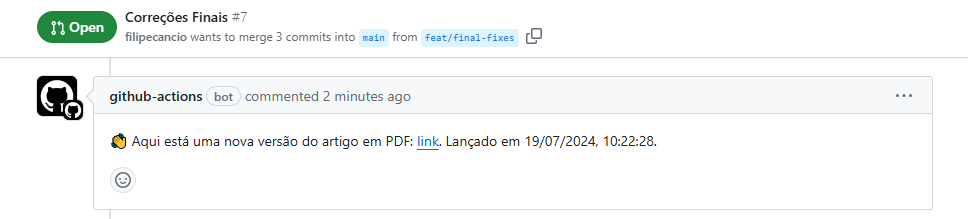
\includegraphics[width=.7\textwidth]{./images/fig06.png}
	\caption{Mensagem do robô do GitHub com link do pdf em Requisições de Pull}
	\label{fig:fig06}
\end{figure}

Com o GitHub Projetos, a edição dos artigos fica ainda mais organizada. É comum na elaboração de artigos em projetos de pesquisa estipular de calendários e cronogramas. No projeto, as próprias Requisições de Pull se tornam o cronograma do artigo, nelas podemos descrever o que será trabalhado de forma completa e documentada, com prazos, legendas e pessoas envolvidas na revisão. É possível inclusive visualizar de três diferentes formas: como tabela (figura~\ref{fig:fig07}), quadros (figura~\ref{fig:fig08}) e gráfico GANTT (figura~\ref{fig:fig09}).

\begin{figure}[H]
	\centering
	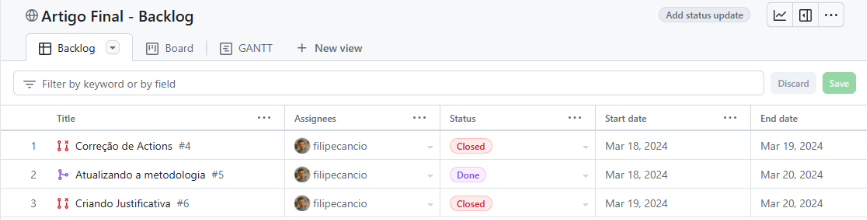
\includegraphics[width=.8\textwidth]{./images/fig07.png}
	\caption{Visualização de Requisições de Pull como tabela no GitHub Projetos}
	\label{fig:fig07}
\end{figure}

\begin{figure}[ht]
	\centering
	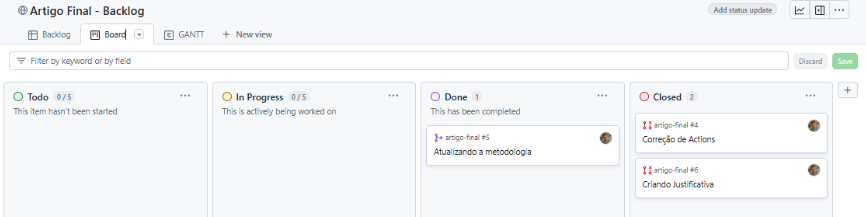
\includegraphics[width=.8\textwidth]{./images/fig08.png}
	\caption{Visualização de Pull Request como quadro no GitHub Projetos}
	\label{fig:fig08}
\end{figure}

\begin{figure}[ht]
	\centering
	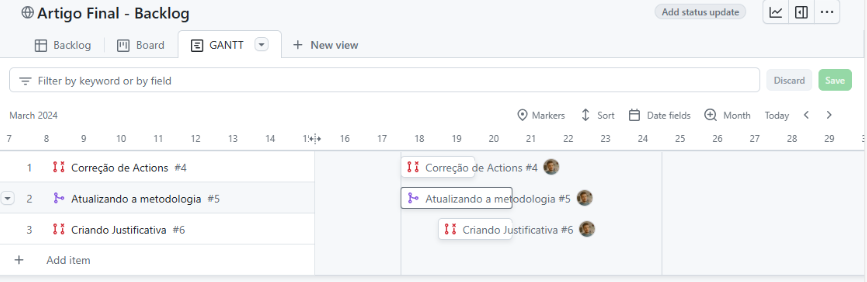
\includegraphics[width=.8\textwidth]{./images/fig09.png}
	\caption{Visualização de Pull Request como GANTT no GitHub Projetos}
	\label{fig:fig09}
\end{figure}

Estes destaques tornam o projeto interessante para a comunidade acadêmica. A possibilidade de manter um artigo no GitHub com registros de alteração de cada parte envolvida também garante proteção contra possíveis fraudes e plágios. É possivel acessar e editar em qualquer plataforma com internet, tornando a escrita acessível a qualquer pessoa na comunidade.

